\documentclass[draft,linenumbers]{agujournal}
\draftfalse
\usepackage{hyperref}
\usepackage[export]{adjustbox}
\addtolength{\oddsidemargin}{-.875in}
\addtolength{\evensidemargin}{-.875in}
	
\hypersetup{
    colorlinks=true,
    linkcolor=blue,
    filecolor=magenta,      
    urlcolor=cyan,
}

\journalname{Journal of Advances in Modeling Earth Systems (JAMES)}

\begin{document}


\begin{figure}[h]
    % \centering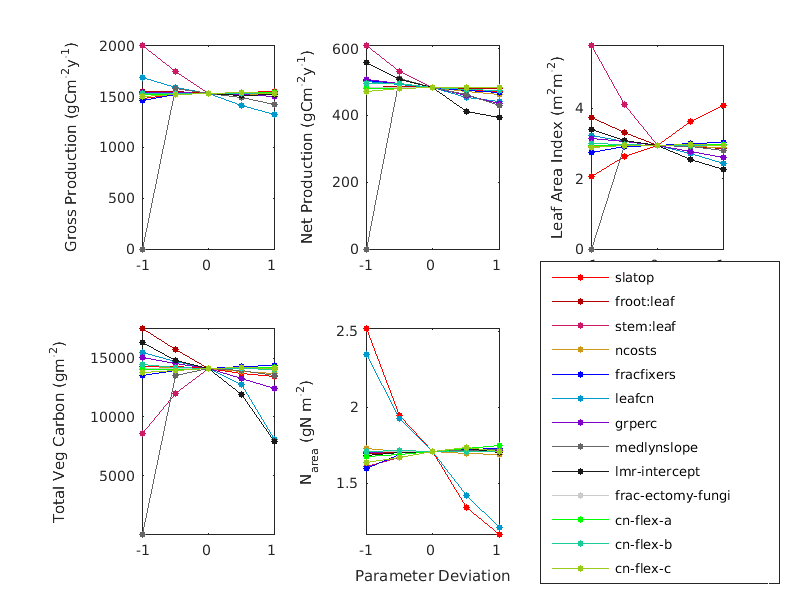
\includegraphics[width=0.5\textwidth, right]{lion-lo9
     \includegraphics[width=1.3\textwidth, left]{matlab/figures/NOVc_STATE_1CLM50defpft_trans_1x1pt_Br-cax_ens_MIC_y1.png}
     \caption{Caxiuana Forest State}
     \label{CAX state}
  \end{figure}
  
 \begin{figure}[h]
    % \centering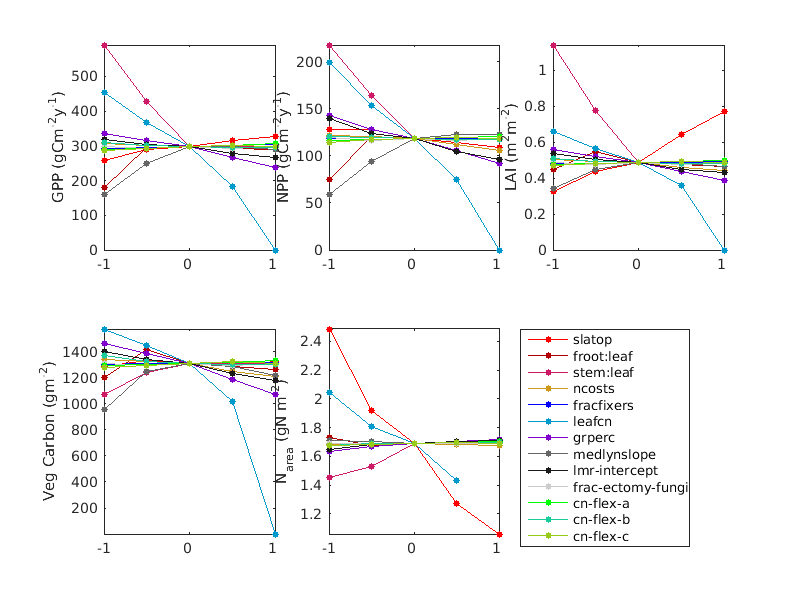
\includegraphics[width=0.5\textwidth, right]{lion-lo9
     \includegraphics[width=1.3\textwidth, left]{matlab/figures/NOVc_STATE_1CLM50defpft_trans_1x1pt_US-Me2_ens_MIC_y1.png}
     \caption{Metolius Forest State}
     \label{MET state}
  \end{figure}
  
   \begin{figure}[h]
    % \centering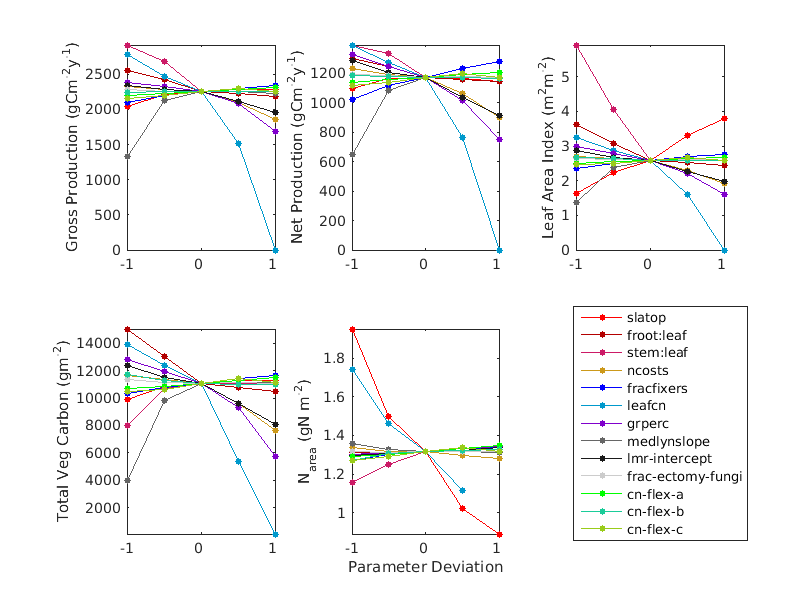
\includegraphics[width=0.5\textwidth, right]{lion-lo9
     \includegraphics[width=1.3\textwidth, left]{matlab/figures/NOVc_STATE_1CLM50defpft_trans_1x1pt_US_Ha1_ens_MIC_y1.png}
     \caption{Harvard Forest State}
     \label{HVF state}
  \end{figure}

 

 \begin{figure}[h]
    % \centering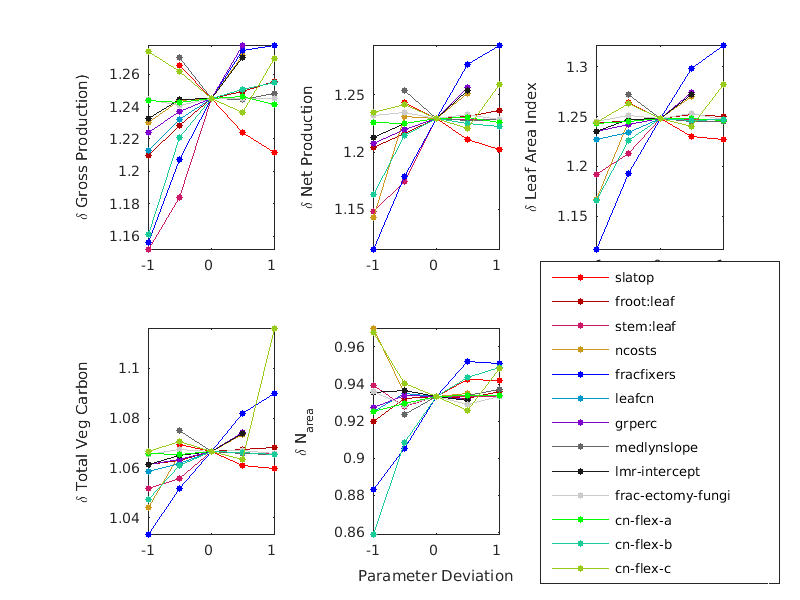
\includegraphics[width=0.5\textwidth, right]{lion-lo9
     \includegraphics[width=1.3\textwidth, left]{matlab/figures/NOVc_FERT_1CLM50defpft_celev_1x1pt_US_Ha1_ens_MIC_p1.png}
     \caption{Harvard Forest Nitrogen Fertilization}
     \label{HRV ndep}
  \end{figure}
  
   \begin{figure}[h]
    % \centering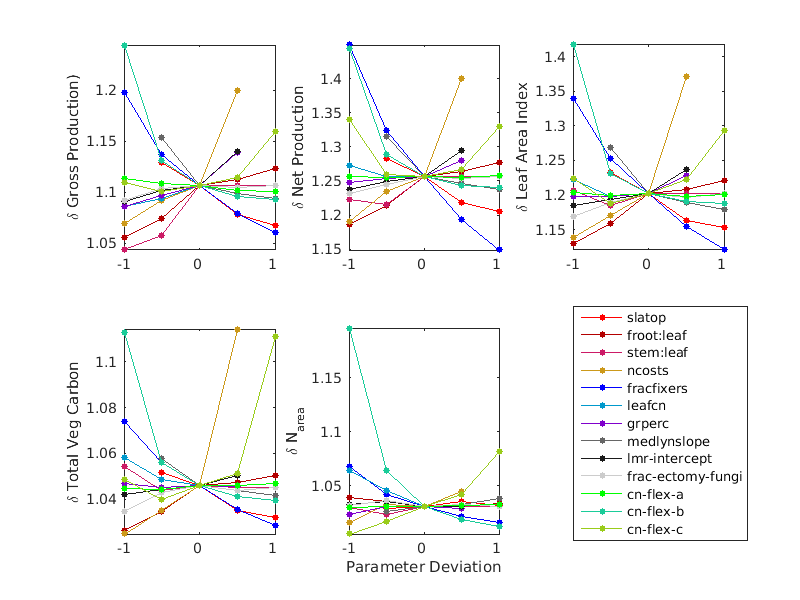
\includegraphics[width=0.5\textwidth, right]{lion-lo9
     \includegraphics[width=1.3\textwidth, left]{matlab/figures/NOVc_FERT_1CLM50defpft_ndep_1x1pt_US_Ha1_ens_MIC_p1.png}
     \caption{Harvard Forest CO2 Fertilization}
     \label{HRV celev}
  \end{figure}
  
   \begin{figure}[h]
    % \centering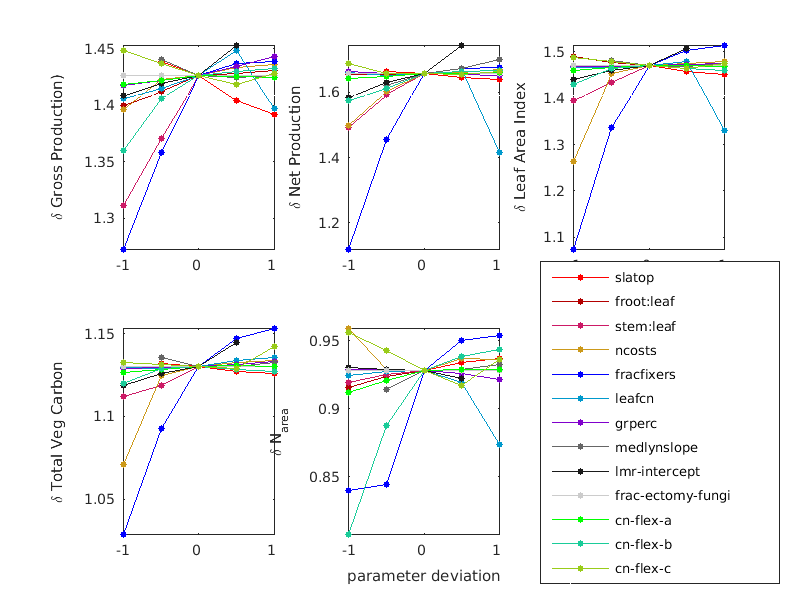
\includegraphics[width=0.5\textwidth, right]{lion-lo9
     \includegraphics[width=1.3\textwidth, left]{matlab/figures/NOVc_FERT_1CLM50defpft_celev_1x1pt_Br-cax_ens_MIC_p1.png}
     \caption{Caxiuana Forest Nitrogen Fertilization}
     \label{CAX ndep}
  \end{figure}
  
   \begin{figure}[h]
    % \centering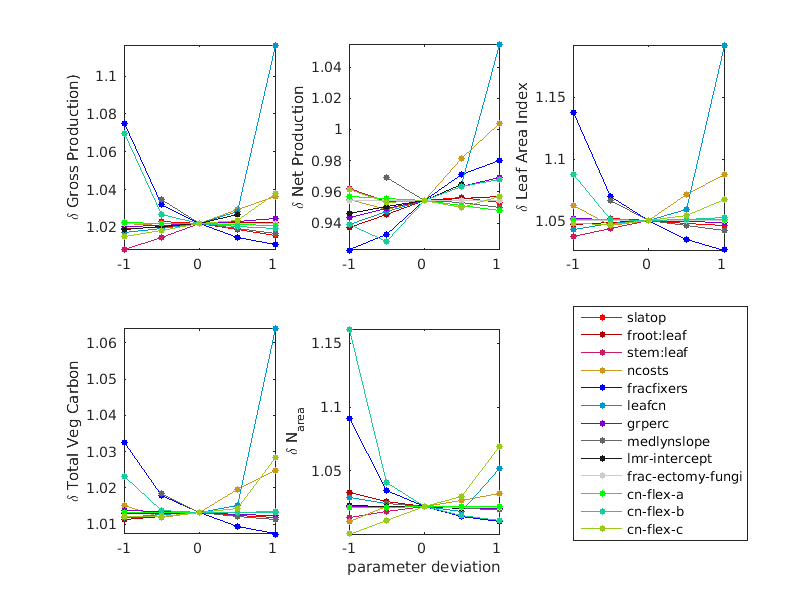
\includegraphics[width=0.5\textwidth, right]{lion-lo9
     \includegraphics[width=1.3\textwidth, left]{matlab/figures/NOVc_FERT_1CLM50defpft_ndep_1x1pt_Br-cax_ens_MIC_p1.png}
     \caption{Caxiuana Forest CO2 Fertilization}
     \label{CAX celev}
  \end{figure}
  
   \begin{figure}[h]
    % \centering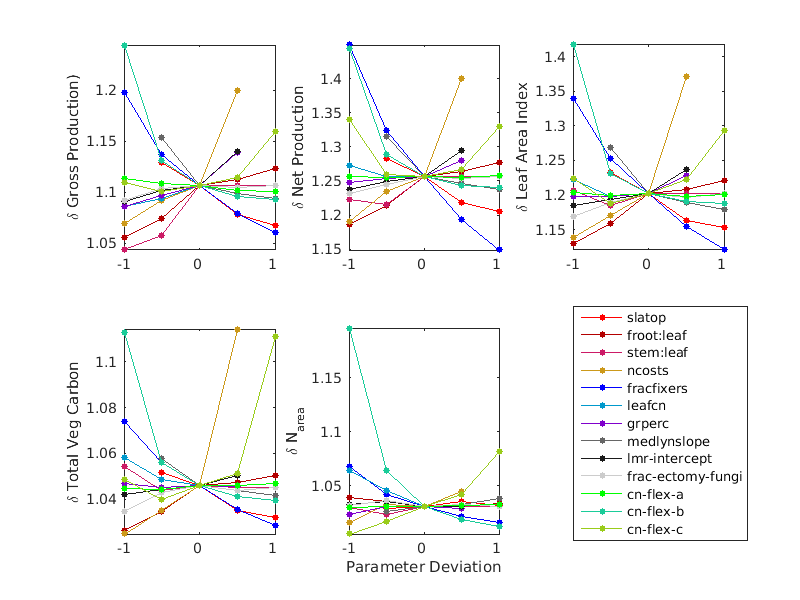
\includegraphics[width=0.5\textwidth, right]{lion-lo9
     \includegraphics[width=1.3\textwidth, left]{matlab/figures/NOVc_FERT_1CLM50defpft_ndep_1x1pt_US_Ha1_ens_MIC_p1.png}
     \caption{Metolius Forest Nitrogen Fertilization}
     \label{MET ndep}
  \end{figure}
  
   \begin{figure}[h]
    % \centering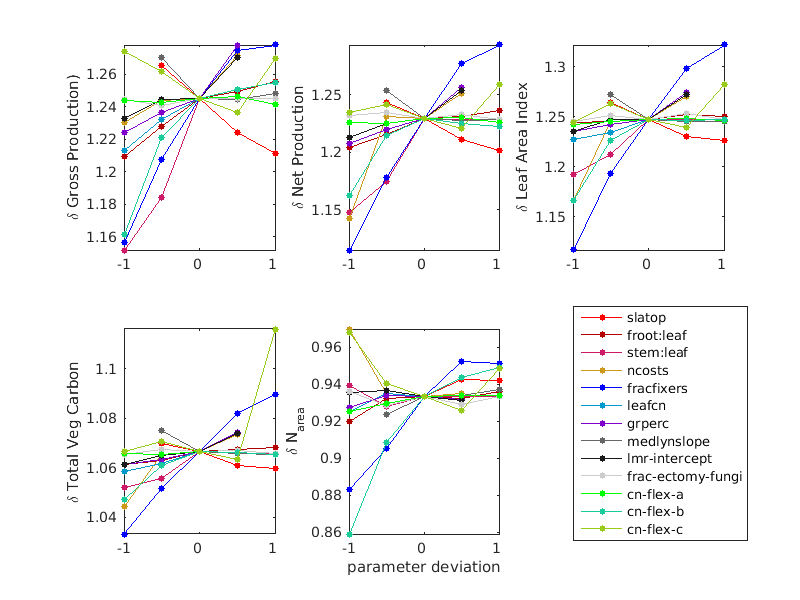
\includegraphics[width=0.5\textwidth, right]{lion-lo9
     \includegraphics[width=1.3\textwidth, left]{matlab/figures/NOVc_FERT_1CLM50defpft_celev_1x1pt_US-Me2_ens_MIC_p1.png}
     \caption{Metolius Forest CO2 Fertilization}
     \label{MET celev}
  \end{figure}
  
   \begin{figure}[h]
    % \centering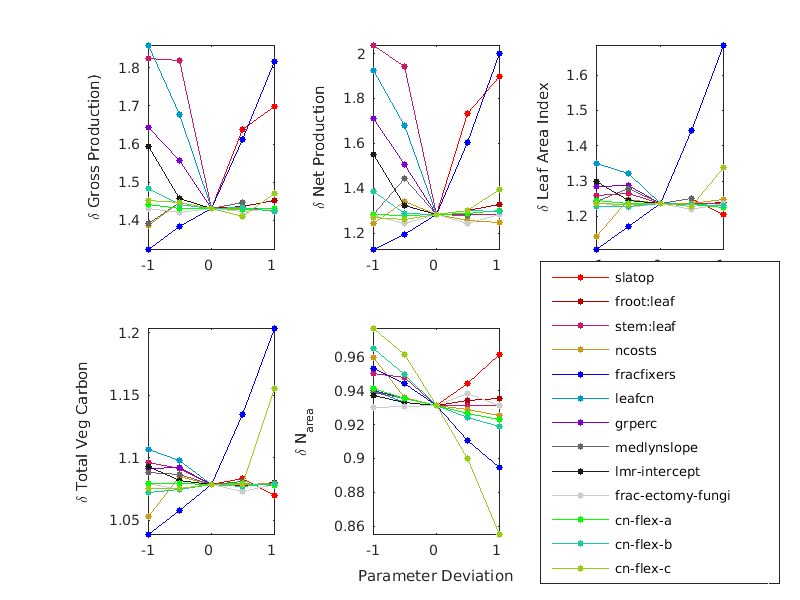
\includegraphics[width=0.5\textwidth, right]{lion-lo9
     \includegraphics[width=1.3\textwidth, left]{matlab/figures/NOVc_FERT_1CLM50defpft_celev_1x1pt_US-NR1_ens_MIC_p1.png}
     \caption{Niwot Forest Nitrogen Fertilization}
     \label{NR1 ndep}
  \end{figure}
  
   \begin{figure}[h]
    % \centering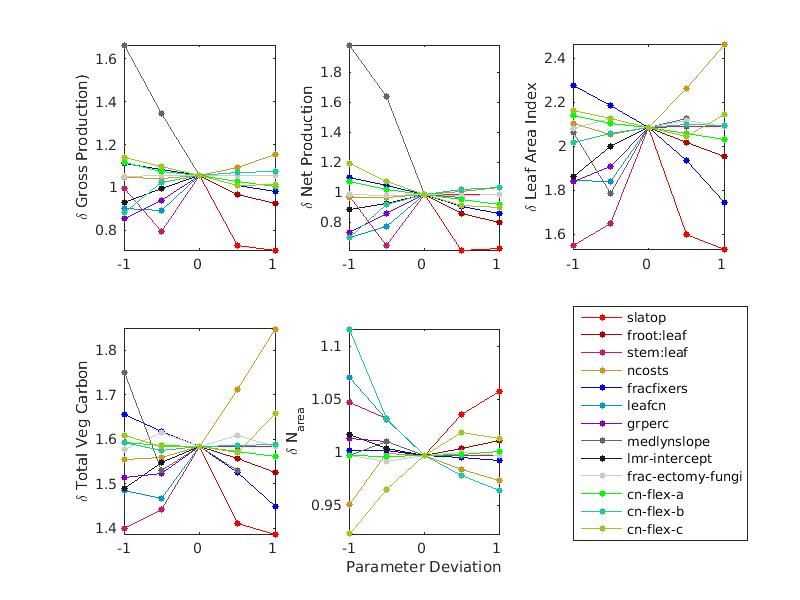
\includegraphics[width=0.5\textwidth, right]{lion-lo9
     \includegraphics[width=1.3\textwidth, left]{matlab/figures/NOVc_FERT_1CLM50defpft_ndep_1x1pt_US-NR1_ens_MIC_p1.png}
     \caption{Niwot Forest CO2 Fertilization}
     \label{NR1 celev}
  \end{figure}

      
 \begin{figure}[h]
     \centering
     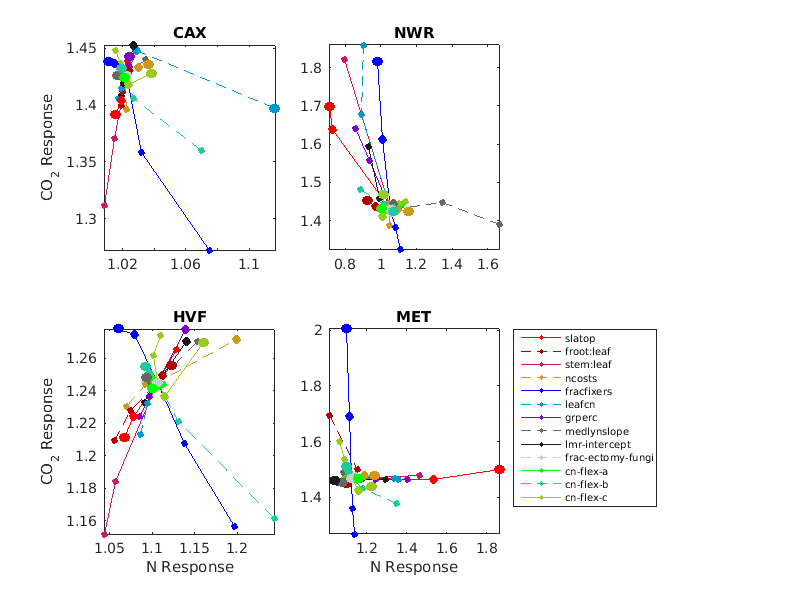
\includegraphics[width=1.55\textwidth, left]{matlab/figures/NOVc_CNdep_GPP1__p2012.png}
     \caption{GPP CO2 and N respones}
     \label{GPP CO2 and N respones 2001}
  \end{figure}
  
 \begin{figure}[h]
     \centering
     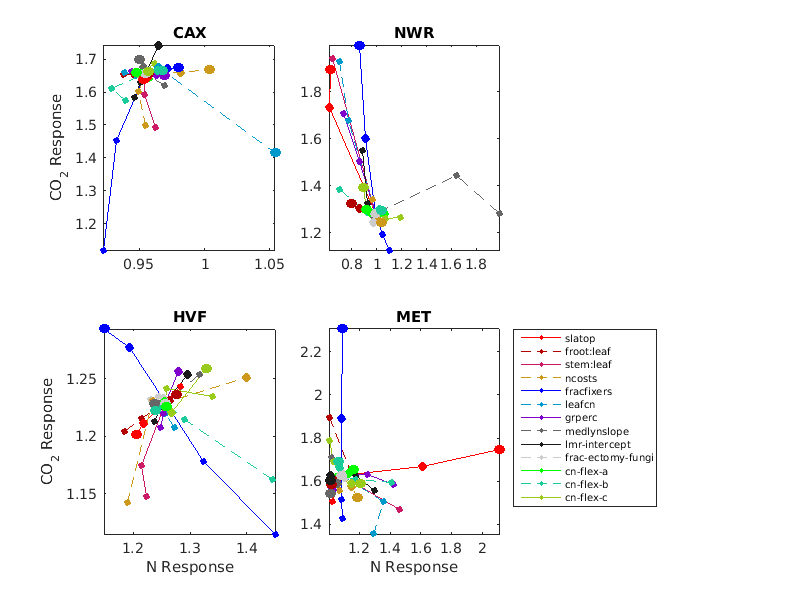
\includegraphics[width=1.55\textwidth, left]{matlab/figures/NOVc_CNdep_NPP1__p2012.png}
     \caption{NPP CO2 and N respones}
     \label{NPP CO2 and N respones 2001}
  \end{figure}
      
 \begin{figure}[h]
     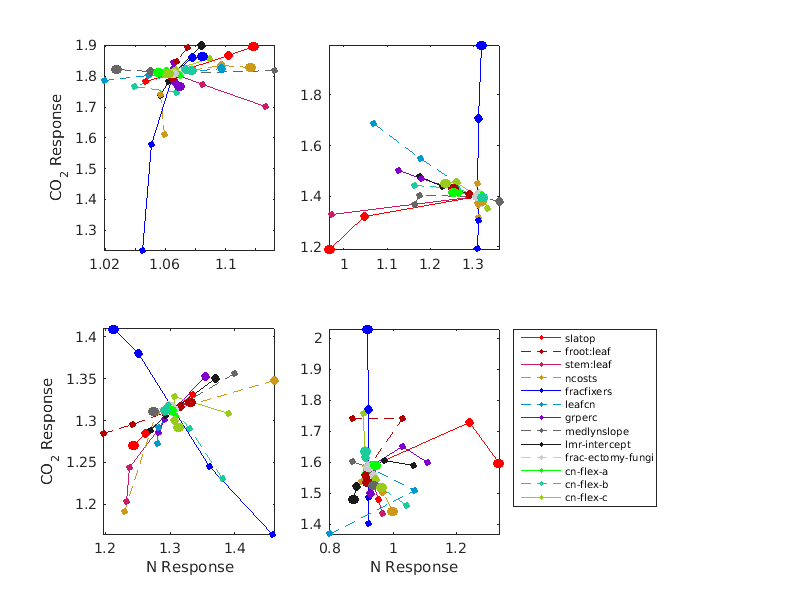
\includegraphics[width=1.55\textwidth, left]{matlab/figures/OCT_CNdep_NPP1_CLM50defpft_ndep_1x1pt_US-Me2_ens_MIC_p2006.png}
     \caption{NPP CO2 and N respones}
     \label{NPP CO2 and N respones}
  \end{figure}
  
   \begin{figure}[h]
     \centering
     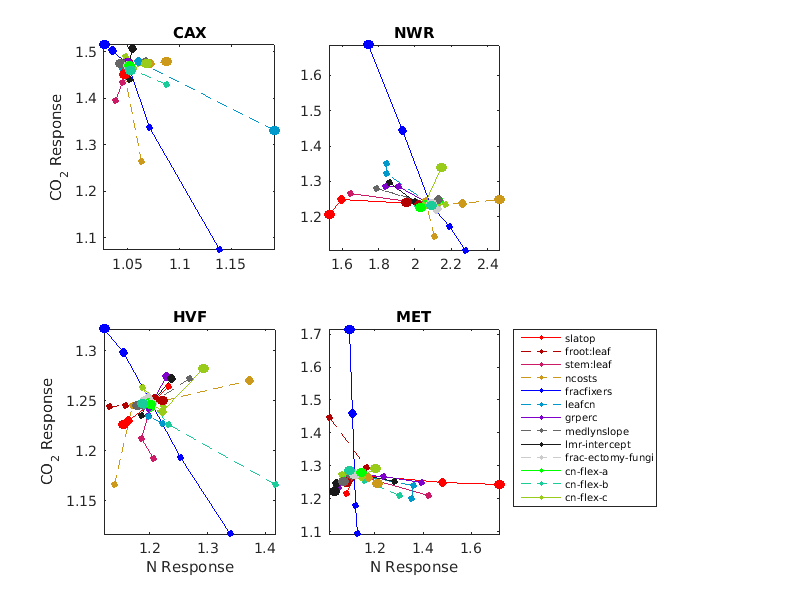
\includegraphics[width=1.55\textwidth, left]{matlab/figures/NOVc_CNdep_TLAI1__p2012.png}
     \caption{LAI CO2 and N respones}
     \label{LAI CO2 and N respones 2001}
  \end{figure}
  
   \begin{figure}[h]
     \centering
     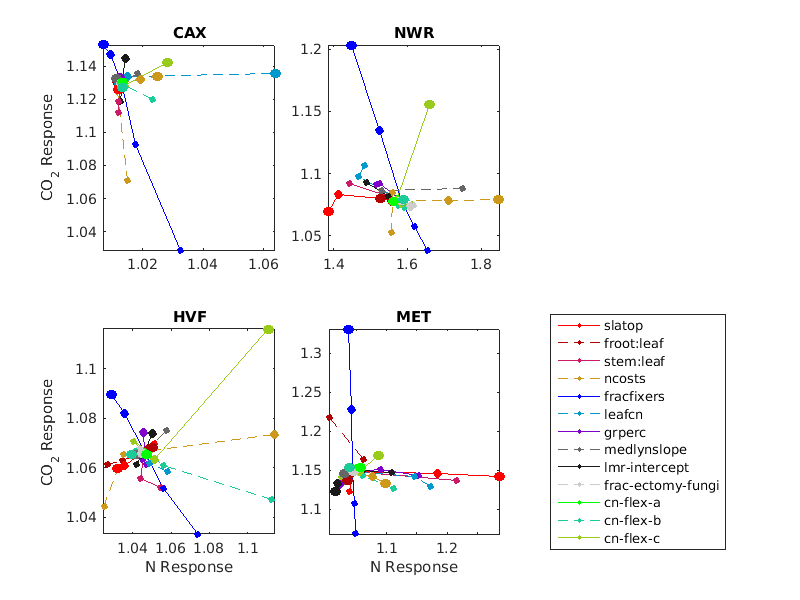
\includegraphics[width=1.55\textwidth, left]{matlab/figures/NOVc_CNdep_TOTVEGC1__p2012.png}
     \caption{VEGC CO2 and N respones}
     \label{VEGC CO2 and N respones 2001}
  \end{figure}
  
   \begin{figure}[h]
     \centering
     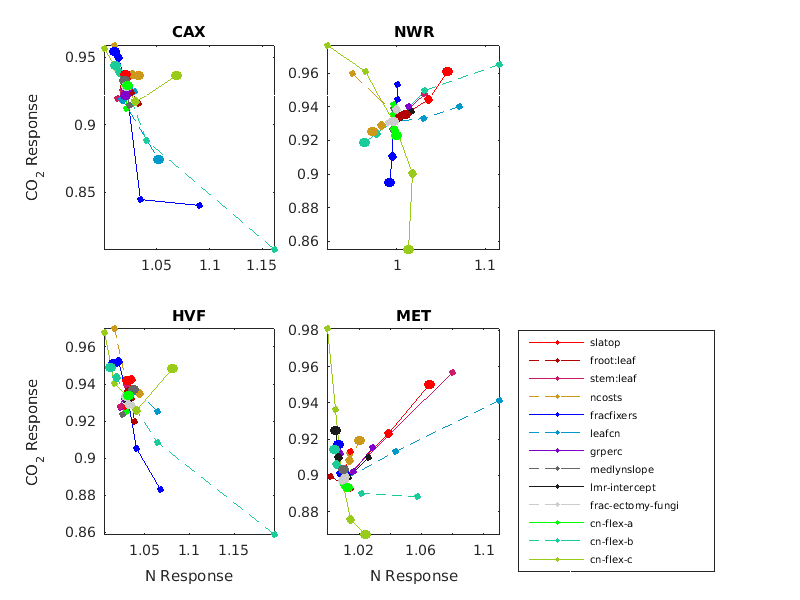
\includegraphics[width=1.55\textwidth, left]{matlab/figures/NOVc_CNdep_LEAFN1__p2012.png}
     \caption{Leaf Nitrogen CO2 and N respones}
     \label{Leaf N CO2 and N respones 2001}
  \end{figure}
    
 
    

  
  
\end{document}